\documentclass[12pt,a4paper]{article}
\usepackage[utf8]{vietnam}
\usepackage{amsmath,amssymb}
\usepackage{tabularx}
\usepackage{tikz}
\usetikzlibrary{calc,angles,quotes,arrows.meta,patterns}
\usepackage{xcolor}
\usepackage{enumitem}
\usepackage{fancyhdr}
\usepackage{graphicx}
\usepackage[top=0.9cm, bottom=0.9cm, left=1.2cm, right=1.2cm]{geometry}
\usepackage[loigiai]{ex_test}
\SAOPTN{widthSA=3.2,heightSA=0.62}

\setlength{\headheight}{15pt}
\setlength{\parskip}{0pt}

\pagestyle{fancy}
\fancyhf{}
\rhead{\textit{Môn Toán 8 -- Hướng dẫn giải Đề số 10}}
\lhead{\textit{Bộ đề ôn tập Giữa học kì I}}
\cfoot{\thepage}

\begin{document}

\begin{center}
  \textbf{\Large HƯỚNG DẪN GIẢI CHI TIẾT VÀ BẢNG ĐÁP ÁN}\\
  \textbf{\large ĐỀ ÔN TẬP GIỮA HỌC KỲ I -- ĐỀ SỐ 10}\\
  \textit{Môn: Toán 8 -- Năm học 2026 -- 2027}
\end{center}
\vspace{2mm}

% --- BẢNG ĐÁP ÁN TRẮC NGHIỆM TÓM TẮT ---
\noindent\textbf{\large A. BẢNG ĐÁP ÁN TRẮC NGHIỆM TỔNG HỢP}
\vspace{1mm}

\noindent\textbf{1. Phần I (Mỗi câu trả lời đúng được 0,25 điểm):}
\begin{center}
\begin{tabular}{|c|c|c|c|c|c|c|c|c|c|c|c|c|}
\hline
\textbf{Câu} & \textbf{1} & \textbf{2} & \textbf{3} & \textbf{4} & \textbf{5} & \textbf{6} & \textbf{7} & \textbf{8} & \textbf{9} & \textbf{10} & \textbf{11} & \textbf{12} \\
\hline
\textbf{Đ/A} & \textbf{A} & \textbf{B} & \textbf{C} & \textbf{A} & \textbf{C} & \textbf{C} & \textbf{B} & \textbf{A} & \textbf{D} & \textbf{A} & \textbf{A} & \textbf{B} \\
\hline
\end{tabular}
\end{center}
\vspace{0.5mm}

\noindent\textbf{2. Phần II (Đúng 1 ý: 0,1đ; 2 ý: 0,25đ; 3 ý: 0,5đ; 4 ý: 1,0đ):}
\begin{center}
\begin{tabular}{|c|c|c|c|c||c|c|c|c|c|}
\hline
\textbf{Câu} & \textbf{a)} & \textbf{b)} & \textbf{c)} & \textbf{d)} & \textbf{Câu} & \textbf{a)} & \textbf{b)} & \textbf{c)} & \textbf{d)} \\
\hline
\textbf{Câu 1} & \textbf{Đ} & \textbf{Đ} & \textbf{Đ} & \textbf{S} & \textbf{Câu 2} & \textbf{Đ} & \textbf{Đ} & \textbf{Đ} & \textbf{S} \\
\hline
\end{tabular}
\end{center}
\vspace{0.5mm}

\noindent\textbf{3. Phần III (Mỗi câu trả lời đúng được 1,0 điểm):}
\begin{center}
\begin{tabular}{|c|c|c|}
\hline
\textbf{Câu} & \textbf{Câu 1} & \textbf{Câu 2} \\
\hline
\textbf{Đáp án} & $\mathbf{13}$ & $\mathbf{(x - y - 3)(x - y + 3)}$ \\
\hline
\end{tabular}
\end{center}
\vspace{1.5mm}

% --- B. LỜI GIẢI CHI TIẾT ---
\noindent\textbf{\large B. LỜI GIẢI CHI TIẾT CÁC CÂU HỎI}
\vspace{1mm}
\begin{ex}
Trong các biểu thức sau, biểu thức nào là đa thức?
\choice
{\True $3x^2 + y$}
{$\dfrac{1}{x}$}
{$-\dfrac{2x + 1}{xy}$}
{$\sqrt{x} - 7$}
\loigiai{
Đa thức là tổng của những đơn thức. Biểu thức $3x^2 + y$ là tổng của hai đơn thức $3x^2$ và $y$ nên là đa thức.
}
\end{ex}

\begin{ex}
Trong các biểu thức sau, biểu thức nào không phải là đơn thức?
\choice
{$\dfrac{1}{4}$}
{\True $2\sqrt{y}$}
{$-3xy^2z^3$}
{$x$}
\loigiai{
Đơn thức là biểu thức đại số chỉ gồm một số, một biến, hoặc một tích giữa các số và các biến. Biểu thức $2\sqrt{y}$ chứa căn bậc hai của biến nên không phải là đơn thức.
}
\end{ex}

\begin{ex}
Bậc của đa thức $x^2y^2 + xy^3 - x^2y^4$ là:
\choice
{3}
{4}
{\True 6}
{8}
\loigiai{
Hạng tử $-x^2y^4$ có tổng số mũ của các biến là $2 + 4 = 6$, đây là hạng tử có bậc cao nhất trong đa thức. Do đó bậc của đa thức bằng 6.
}
\end{ex}

\begin{ex}
Đơn thức $12x^5y^4$ chia hết cho đơn thức nào dưới đây?
\choice
{\True $5x^2y$}
{$6x^5y^5$}
{$2x^2yz$}
{$3x^5y^6$}
\loigiai{
Đơn thức $12x^5y^4$ chia hết cho $5x^2y$ vì số mũ của mỗi biến trong $5x^2y$ đều nhỏ hơn hoặc bằng số mũ của biến tương ứng trong $12x^5y^4$.
}
\end{ex}

\begin{ex}
Cho tứ giác $ABCD$ biết $\widehat{A} = 33^\circ, \widehat{B} = 122^\circ, \widehat{C} = 78^\circ$. Khi đó số đo góc $\widehat{D}$ là:
\choice
{$66^\circ$}
{$142^\circ$}
{\True $127^\circ$}
{$33^\circ$}
\loigiai{
Tổng số đo bốn góc trong một tứ giác bằng $360^\circ$. Ta có: $\widehat{D} = 360^\circ - 33^\circ - 122^\circ - 78^\circ = 127^\circ$.
}
\end{ex}

\begin{ex}
Đơn thức $-\dfrac{1}{5}x^2y^3(-5x^3y)ax$ với $a$ là hằng số có hệ số và bậc lần lượt là:
\choice
{$a$ và $6$}
{$1$ và $10$}
{\True $a$ và $10$}
{$1$ và $6$}
\loigiai{
Thu gọn đơn thức: $-\dfrac{1}{5}x^2y^3 \cdot (-5x^3y) \cdot ax = ax^6y^4$. Hệ số là $a$ và bậc là $6 + 4 = 10$.
}
\end{ex}

\begin{ex}
Cặp đơn thức nào sau đây là đồng dạng với nhau?
\choice
{$\dfrac{1}{2}x^2y$ và $2xy^2$}
{\True $-x^2y^4$ và $2x^2y^4$}
{$6yt$ và $26y$}
{$mxy$ và $ny^2$ với $m, n$ là hằng số khác $0$}
\loigiai{
Hai đơn thức đồng dạng có hệ số khác 0 và có cùng phần biến. Cặp đơn thức $-x^2y^4$ và $2x^2y^4$ có cùng phần biến $x^2y^4$.
}
\end{ex}

\begin{ex}
Hình bình hành cần có thêm điều kiện nào sau đây thì trở thành hình chữ nhật?
\choice
{\True Có một góc vuông}
{Có hai cạnh kề bằng nhau}
{Có hai đường chéo vuông góc}
{Có hai đường chéo cắt nhau tại trung điểm mỗi đường}
\loigiai{
Theo dấu hiệu nhận biết, hình bình hành có một góc vuông là hình chữ nhật.
}
\end{ex}

\begin{ex}
Hình bình hành $ABCD$ có $\widehat{A} = 65^\circ$. Số đo góc $\widehat{C}$ là:
\choice
{$125^\circ$}
{$95^\circ$}
{$115^\circ$}
{\True $65^\circ$}
\loigiai{
Trong hình bình hành, hai góc đối bằng nhau nên $\widehat{C} = \widehat{A} = 65^\circ$.
}
\end{ex}

\begin{ex}
Cho tam giác $ABC$ vuông tại $A$ có $M$ là trung điểm của $BC$, biết $BC = 10\text{ cm}$. Khi đó độ dài $AM$ bằng:
\choice
{\True $5\text{ cm}$}
{$10\text{ cm}$}
{$2{,}5\text{ cm}$}
{$20\text{ cm}$}
\loigiai{
Trong tam giác vuông, đường trung tuyến ứng với cạnh huyền bằng nửa cạnh huyền: $AM = \dfrac{BC}{2} = \dfrac{10}{2} = 5\text{ cm}$.
}
\end{ex}

\begin{ex}
Hình nào sau đây có hai đường chéo không cắt nhau tại trung điểm của mỗi đường?
\choice
{\True Hình thang cân}
{Hình bình hành}
{Hình chữ nhật}
{Hình vuông}
\loigiai{
Hình thang cân nói chung không có tính chất hai đường chéo cắt nhau tại trung điểm mỗi đường. Tính chất này thuộc về hình bình hành và các dạng đặc biệt của nó.
}
\end{ex}

\begin{ex}
Thể tích của hình chóp tam giác đều có diện tích đáy bằng $9\text{ cm}^2$ và chiều cao bằng $4\text{ cm}$ là:
\choice
{$36\text{ cm}^3$}
{\True $12\text{ cm}^3$}
{$27\text{ cm}^3$}
{$13\text{ cm}^3$}
\loigiai{
Thể tích hình chóp tam giác đều: $V = \dfrac{1}{3} S \cdot h = \dfrac{1}{3} \cdot 9 \cdot 4 = 12\text{ cm}^3$.
}
\end{ex}


\setcounter{ex}{0}
\noindent\textbf{\large PHẦN II. CÂU TRẮC NGHIỆM ĐÚNG SAI}
\vspace{1mm}
\begin{ex}
Cho biểu thức $A = (x + 2)^3 - x(x + 1)(x - 1) - 6x^2$. Xét tính đúng sai của các mệnh đề sau:
\choiceTF
{\True Khai triển hằng đẳng thức $(x + 2)^3$ ta được $x^3 + 6x^2 + 12x + 8$}
{\True Kết quả của tích $x(x + 1)(x - 1)$ là $x^3 - x$}
{\True Kết quả rút gọn của biểu thức $A$ là $13x + 8$}
{Tại $x = -1$, giá trị của biểu thức $A$ bằng $5$}
\loigiai{
\textbf{a)} \textbf{Đúng.} $(x + 2)^3 = x^3 + 3 \cdot x^2 \cdot 2 + 3 \cdot x \cdot 2^2 + 2^3 = x^3 + 6x^2 + 12x + 8$.

\textbf{b)} \textbf{Đúng.} $x(x + 1)(x - 1) = x(x^2 - 1) = x^3 - x$.

\textbf{c)} \textbf{Đúng.} $A = (x^3 + 6x^2 + 12x + 8) - (x^3 - x) - 6x^2 = 13x + 8$.

\textbf{d)} \textbf{Sai.} Thay $x = -1$ vào: $A = 13(-1) + 8 = -5 \neq 5$.
}
\end{ex}

\begin{ex}
Cho hình thoi $ABCD$ có $\widehat{A} = 60^\circ$ và độ dài cạnh $AB = 4\text{ cm}$. Hai đường chéo $AC$ và $BD$ cắt nhau tại $O$. Xét tính đúng sai của các mệnh đề sau:
\choiceTF
{\True Tam giác $ABD$ là tam giác đều}
{\True Độ dài đường chéo $BD$ bằng $4\text{ cm}$}
{\True Hai đường chéo $AC$ và $BD$ vuông góc với nhau tại trung điểm $O$}
{Độ dài đoạn thẳng $AO$ bằng $2\text{ cm}$}
\loigiai{
\textbf{a)} \textbf{Đúng.} Tam giác $ABD$ có $AB = AD$ và $\widehat{A} = 60^\circ$ nên là tam giác đều.

\textbf{b)} \textbf{Đúng.} Vì tam giác $ABD$ đều nên $BD = AB = 4\text{ cm}$.

\textbf{c)} \textbf{Đúng.} Theo tính chất hình thoi, hai đường chéo vuông góc với nhau tại trung điểm mỗi đường.

\textbf{d)} \textbf{Sai.} $AO$ là đường cao của tam giác đều $ABD$ cạnh $4\text{ cm}$, do đó $AO = \dfrac{4\sqrt{3}}{2} = 2\sqrt{3}\text{ cm} \neq 2\text{ cm}$.
}
\end{ex}


\setcounter{ex}{0}
\noindent\textbf{\large PHẦN III. CÂU HỎI TRẢ LỜI NGẮN}
\vspace{1mm}
\begin{ex}
Cho $x + y = 5$ và $xy = 6$. Tính giá trị của biểu thức $A = x^2 + y^2$. \shortans{13}
\loigiai{
Ta có: $A = x^2 + y^2 = (x + y)^2 - 2xy$.

Thay $x + y = 5$ và $xy = 6$ vào biểu thức, ta được: $A = 5^2 - 2 \cdot 6 = 25 - 12 = 13$.
}
\end{ex}

\begin{ex}
Phân tích đa thức sau thành nhân tử: $x^2 - 2xy + y^2 - 9$. \shortans{$(x - y - 3)(x - y + 3)$}
\loigiai{
Ta có: $x^2 - 2xy + y^2 - 9 = (x - y)^2 - 3^2 = (x - y - 3)(x - y + 3)$.
}
\end{ex}


\setcounter{ex}{0}
\noindent\textbf{\large PHẦN IV. TỰ LUẬN (HƯỚNG DẪN GIẢI VÀ THANG ĐIỂM)}
\vspace{1mm}
\begin{ex} (1,0 điểm)
Thực hiện các phép tính sau:
\begin{enumerate}[label=\textbf{\alph*)}, leftmargin=0.8cm, itemsep=0pt, topsep=1pt]
\item (0,35 điểm) $-3x(x^2y + 2y^2) + 3x^3y$
\item (0,35 điểm) $(x + 2y)^2 + (x + 2y)(x - 2y) - 4xy$
\item (0,3 điểm) $(x - 1)^3 + 3(x + 2)^2 - x(x + 1)(x - 1)$
\end{enumerate}
\loigiai{
\textbf{a)} \textit (0,35 điểm): $-3x(x^2y + 2y^2) + 3x^3y = -3x^3y - 6xy^2 + 3x^3y = -6xy^2$.

\textbf{b)} \textit (0,35 điểm): $(x + 2y)^2 + (x + 2y)(x - 2y) - 4xy = (x^2 + 4xy + 4y^2) + (x^2 - 4y^2) - 4xy = 2x^2$.

\textbf{c)} \textit (0,3 điểm): $(x - 1)^3 + 3(x + 2)^2 - x(x^2 - 1) = (x^3 - 3x^2 + 3x - 1) + 3(x^2 + 4x + 4) - (x^3 - x) = 16x + 11$.


}
\end{ex}
\vspace{0.5mm}

\begin{ex} (0,75 điểm)
Tìm $x$, biết:
\begin{enumerate}[label=\textbf{\alph*)}, leftmargin=0.8cm, itemsep=0pt, topsep=1pt]
\item (0,35 điểm) $3x(x + 2) - 3x^2 = 18$
\item (0,4 điểm) $(x + 1)^2 - (x - 3)(x + 3) = 10$
\end{enumerate}
\loigiai{
\textbf{a)} \textit (0,35 điểm): $3x(x + 2) - 3x^2 = 18 \Leftrightarrow 3x^2 + 6x - 3x^2 = 18 \Leftrightarrow 6x = 18 \Leftrightarrow x = 3$.

\textbf{b)} \textit (0,4 điểm): $(x + 1)^2 - (x - 3)(x + 3) = 10 \Leftrightarrow (x^2 + 2x + 1) - (x^2 - 9) = 10 \Leftrightarrow 2x + 10 = 10 \Leftrightarrow 2x = 0 \Leftrightarrow x = 0$.


}
\end{ex}
\vspace{0.5mm}

\begin{ex} (0,75 điểm)
Cho tam giác $ABC$ vuông tại $A$ có đường cao $AH$. Từ $H$ kẻ $HN \perp AC, HM \perp AB$.
\begin{center}
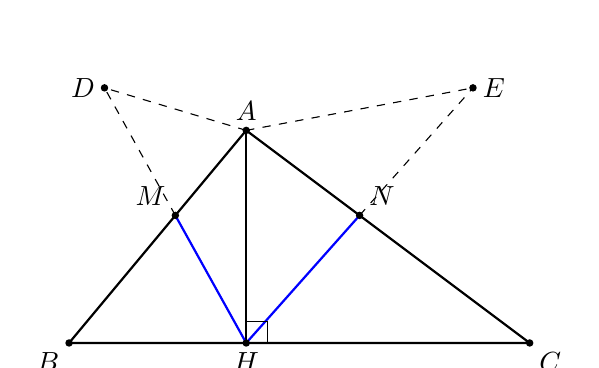
\begin{tikzpicture}[scale=0.9, >=stealth]
  \coordinate (A) at (0,3);
  \coordinate (B) at (-2.5,0);
  \coordinate (C) at (4,0);
  \coordinate (H) at (0,0);
  \coordinate (M) at ($(A)!0.4!(B)$);
  \coordinate (N) at ($(A)!0.4!(C)$);
  \coordinate (D) at ($(M)!-1!(H)$);
  \coordinate (E) at ($(N)!-1!(H)$);
  \draw[thick] (A)--(B)--(C)--cycle;
  \draw[thick] (A)--(H);
  \draw[thick, blue] (H)--(M);
  \draw[thick, blue] (H)--(N);
  \draw[dashed] (M)--(D) (N)--(E);
  \draw[dashed] (A)--(D) (A)--(E);
  \fill (A) circle (1.5pt) node[above] {$A$};
  \fill (B) circle (1.5pt) node[below left] {$B$};
  \fill (C) circle (1.5pt) node[below right] {$C$};
  \fill (H) circle (1.5pt) node[below] {$H$};
  \fill (M) circle (1.5pt) node[above left] {$M$};
  \fill (N) circle (1.5pt) node[above right] {$N$};
  \fill (D) circle (1.5pt) node[left] {$D$};
  \fill (E) circle (1.5pt) node[right] {$E$};
  \draw (0,0.3) -| (0.3,0);
\end{tikzpicture}
\end{center}
\begin{enumerate}[label=\textbf{\alph*)}, leftmargin=0.8cm, itemsep=0pt, topsep=1pt]
\item (0,25 điểm) Chứng minh tứ giác $AMHN$ là hình chữ nhật.
\item (0,25 điểm) Lấy điểm $D$ sao cho $M$ là trung điểm của $DH$, lấy điểm $E$ sao cho $N$ là trung điểm của $EH$. Chứng minh $AD = AE$.
\item (0,25 điểm) Chứng minh $BC^2 = BD^2 + CE^2 + 2BH \cdot HC$.
\end{enumerate}
\loigiai{
\textbf{a)} \textit (0,25 điểm): Tứ giác $AMHN$ có $\widehat{MAN} = 90^\circ$ (do $\Delta ABC$ vuông tại $A$), $\widehat{AMH} = 90^\circ$ (do $HM \perp AB$) và $\widehat{ANH} = 90^\circ$ (do $HN \perp AC$). Tứ giác có 3 góc vuông nên $AMHN$ là hình chữ nhật.

\textbf{b)} \textit (0,25 điểm): Vì $HM \perp AB$ tại trung điểm $M$ của $DH$ nên $AB$ là đường trung trực của $DH \Rightarrow AD = AH$. Tương tự, $AC$ là đường trung trực của $EH \Rightarrow AE = AH$. Do đó $AD = AE$ ($= AH$).

\textbf{c)} \textit (0,25 điểm): Vì $AB$ là đường trung trực của $DH$ nên $BD = BH$. Tương tự, $AC$ là đường trung trực của $EH$ nên $CE = CH$. Ta có: $BC^2 = (BH + HC)^2 = BH^2 + HC^2 + 2BH \cdot HC$. Thay $BH = BD$ và $HC = CE$, ta được: $BC^2 = BD^2 + CE^2 + 2BH \cdot HC$.


}
\end{ex}
\vspace{0.5mm}

\begin{ex} (0,5 điểm)
Tìm đa thức $P(x)$ biết rằng $P(x)$ chia cho $x - 3$ dư 7; chia cho $x - 2$ dư 5; chia cho $(x - 2)(x - 3)$ được thương là $3x$ và còn dư.
\begin{enumerate}[label=\textbf{\alph*)}, leftmargin=0.8cm, itemsep=0pt, topsep=1pt]
\item (0,5 điểm) Tìm đa thức $P(x)$.
\end{enumerate}
\loigiai{
\textbf{a)} \textit (0,5 điểm): Vì chia cho đa thức bậc hai $(x - 2)(x - 3)$ nên phần dư có dạng $R(x) = ax + b$.

Biểu diễn: $P(x) = 3x(x - 2)(x - 3) + ax + b$.

- $P(x)$ chia cho $x - 3$ dư 7 nên $P(3) = 7 \Rightarrow 3a + b = 7$ (1).

- $P(x)$ chia cho $x - 2$ dư 5 nên $P(2) = 5 \Rightarrow 2a + b = 5$ (2).

Lấy (1) trừ (2) ta được: $a = 2$. Thay vào (2) suy ra $b = 1$.

Do đó phần dư là $R(x) = 2x + 1$.

Đa thức cần tìm là:
$P(x) = 3x(x^2 - 5x + 6) + 2x + 1 = 3x^3 - 15x^2 + 18x + 2x + 1 = 3x^3 - 15x^2 + 20x + 1$.


}
\end{ex}
\vspace{0.5mm}


\enlargethispage{1.5cm}
\begin{center}
\rule{4cm}{0.4pt}\\
\textit{--- HẾT ---}
\end{center}
\end{document}
